% !TEX root = ../main.tex
% --+ 12.11 SUMMARY +-----------------------------------------------------------
\begin{frame}{Phase Space Study}
    \label{12.11::summary}

    To select the region where to place the target, a phase space study was conducted.

    \vspace{12pt}
    \begin{itemize}
        \item
            The RG-F target gas region (\ef{$-30 < v_z < 20$ cm}) was divided into ten 5 cm bins.

        \vspace{6pt}
        \item
            The phase space of each relevant kinematic variable (\ef{$Q^2$}, \ef{$\nu$}, \ef{$z_h$}, \ef{$p_T^2$}, \ef{$\phi_{PQ}$}) was analysed for each bin.

        \vspace{6pt}
        \item
            The objective is to \ef{find a region that maximises each phase space}.

        \vspace{6pt}
        \item
            The error bars shown are the quadratic addition of the measurement and acceptance errors\appref{20.09::study_error_estimation}.
    \end{itemize}
\end{frame}

% --+ 12.12 Q2 +----------------------------------------------------------------
\begin{frame}{Phase Space Study: $Q^2$}
    \label{12.12::q2}

    \begin{columns}[onlytextwidth,T]

    \begin{column}{.80\linewidth}
        \vspace{-15pt}
        \begin{center}
            \begin{figure}[t]
                \centering{
                    \fbox{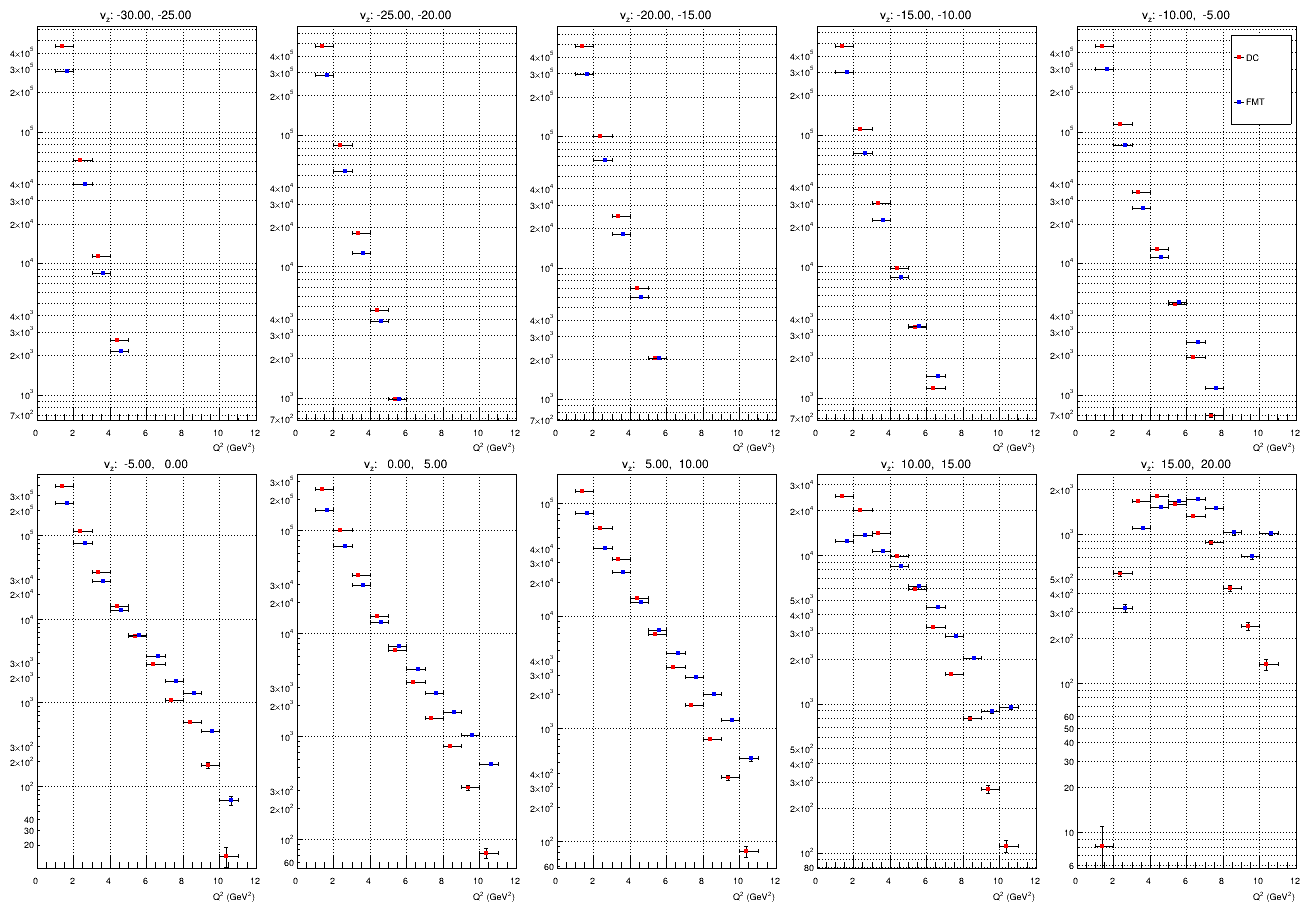
\includegraphics[width=\textwidth]{12q2.png}}
                }
            \end{figure}
        \end{center}
    \end{column}

    \begin{column}{.18\linewidth}
        \vspace{27pt}

        \small{\ef{$v_z < -5$ cm:} \\ higher end of the phase space is limited.}

        \vspace{12pt}

        \small{\ef{$v_z > 15$ cm:} \\ $Q^2$ has an unusual shape.}

        \vspace{12pt}

        \small{\ef{Both effects are attributed to the FMT acceptance region.}}
    \end{column}

    \end{columns}
\end{frame}

